% ----------------------------------------------------------
\section{Hasil Pengujian}
% ----------------------------------------------------------
Bagian ini menyajikan hasil eksperimen model CNN serta RNN/LSTM yang dijalankan melalui Jupyter Notebook. Pengujian mencakup variasi arsitektur, parameter pelatihan, hingga perbandingan performa dengan pustaka standar Keras sebagai \textit{benchmark}.

\subsection{CNN}

Berdasarkan hasil eksperimen pencarian parameter (\textit{hyperparameter sweep}) 16 konfigurasi menggunakan pustaka Keras, diperoleh analisis dari berbagai komponen variasi arsitektur CNN sebagai berikut. Parameter performa utama yang diukur adalah F1-Score (\textit{Macro}) pada himpunan data uji (\textit{test set}) dan waktu pelatihan model.

\subsubsection{Pengaruh Jumlah Layer Konvolusi}
Peningkatan kedalaman arsitektur dari 2 layer menjadi 3 layer secara signifikan meningkatkan performa model (F1-Macro naik dari 0.7607 menjadi 0.8058). Hal ini menunjukkan bahwa arsitektur yang lebih dalam mampu mengekstraksi representasi fitur hierarkis yang lebih kompleks. Namun, penambahan layer ini juga mengakibatkan peningkatan beban komputasi pelatihan, dari rata-rata 110.07 detik menjadi 181.56 detik.

\begin{figure}[H]
    \centering
    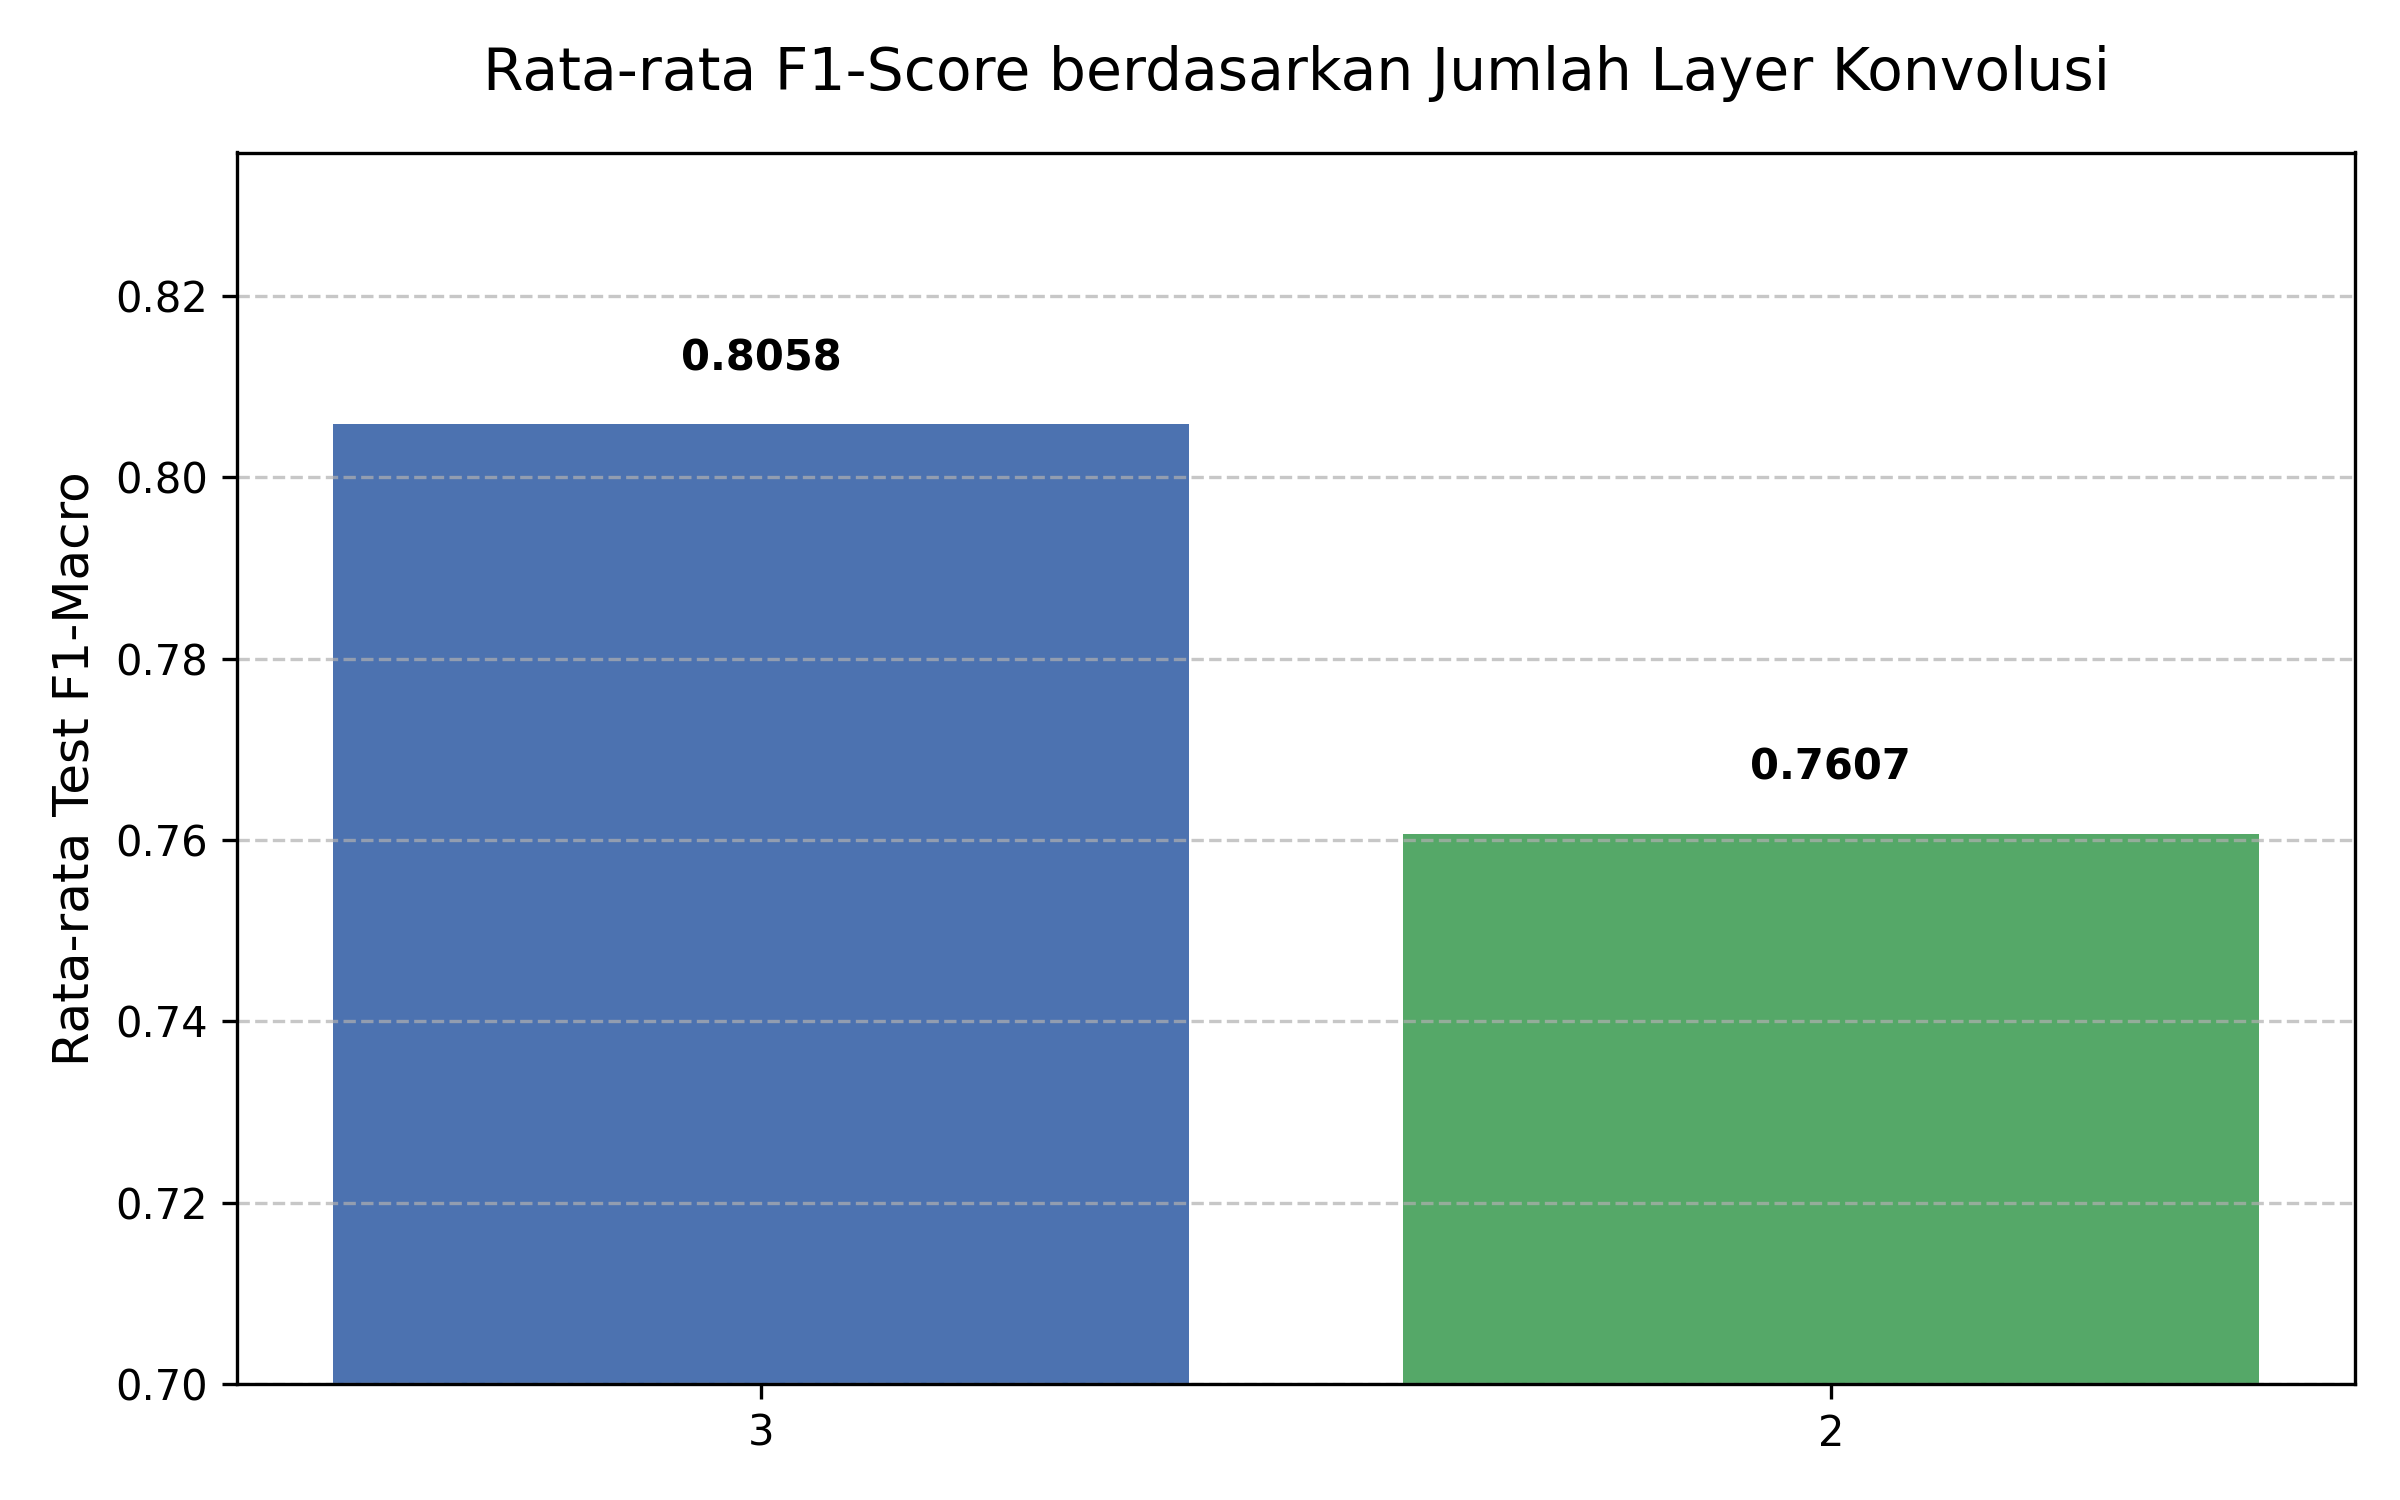
\includegraphics[width=0.7\textwidth]{assets/plot_laporan/1_F1_Jumlah_Layer.png}
    \caption{Rata-rata F1-Score berdasarkan Jumlah Layer}
\end{figure}
\begin{figure}[H]
    \centering
    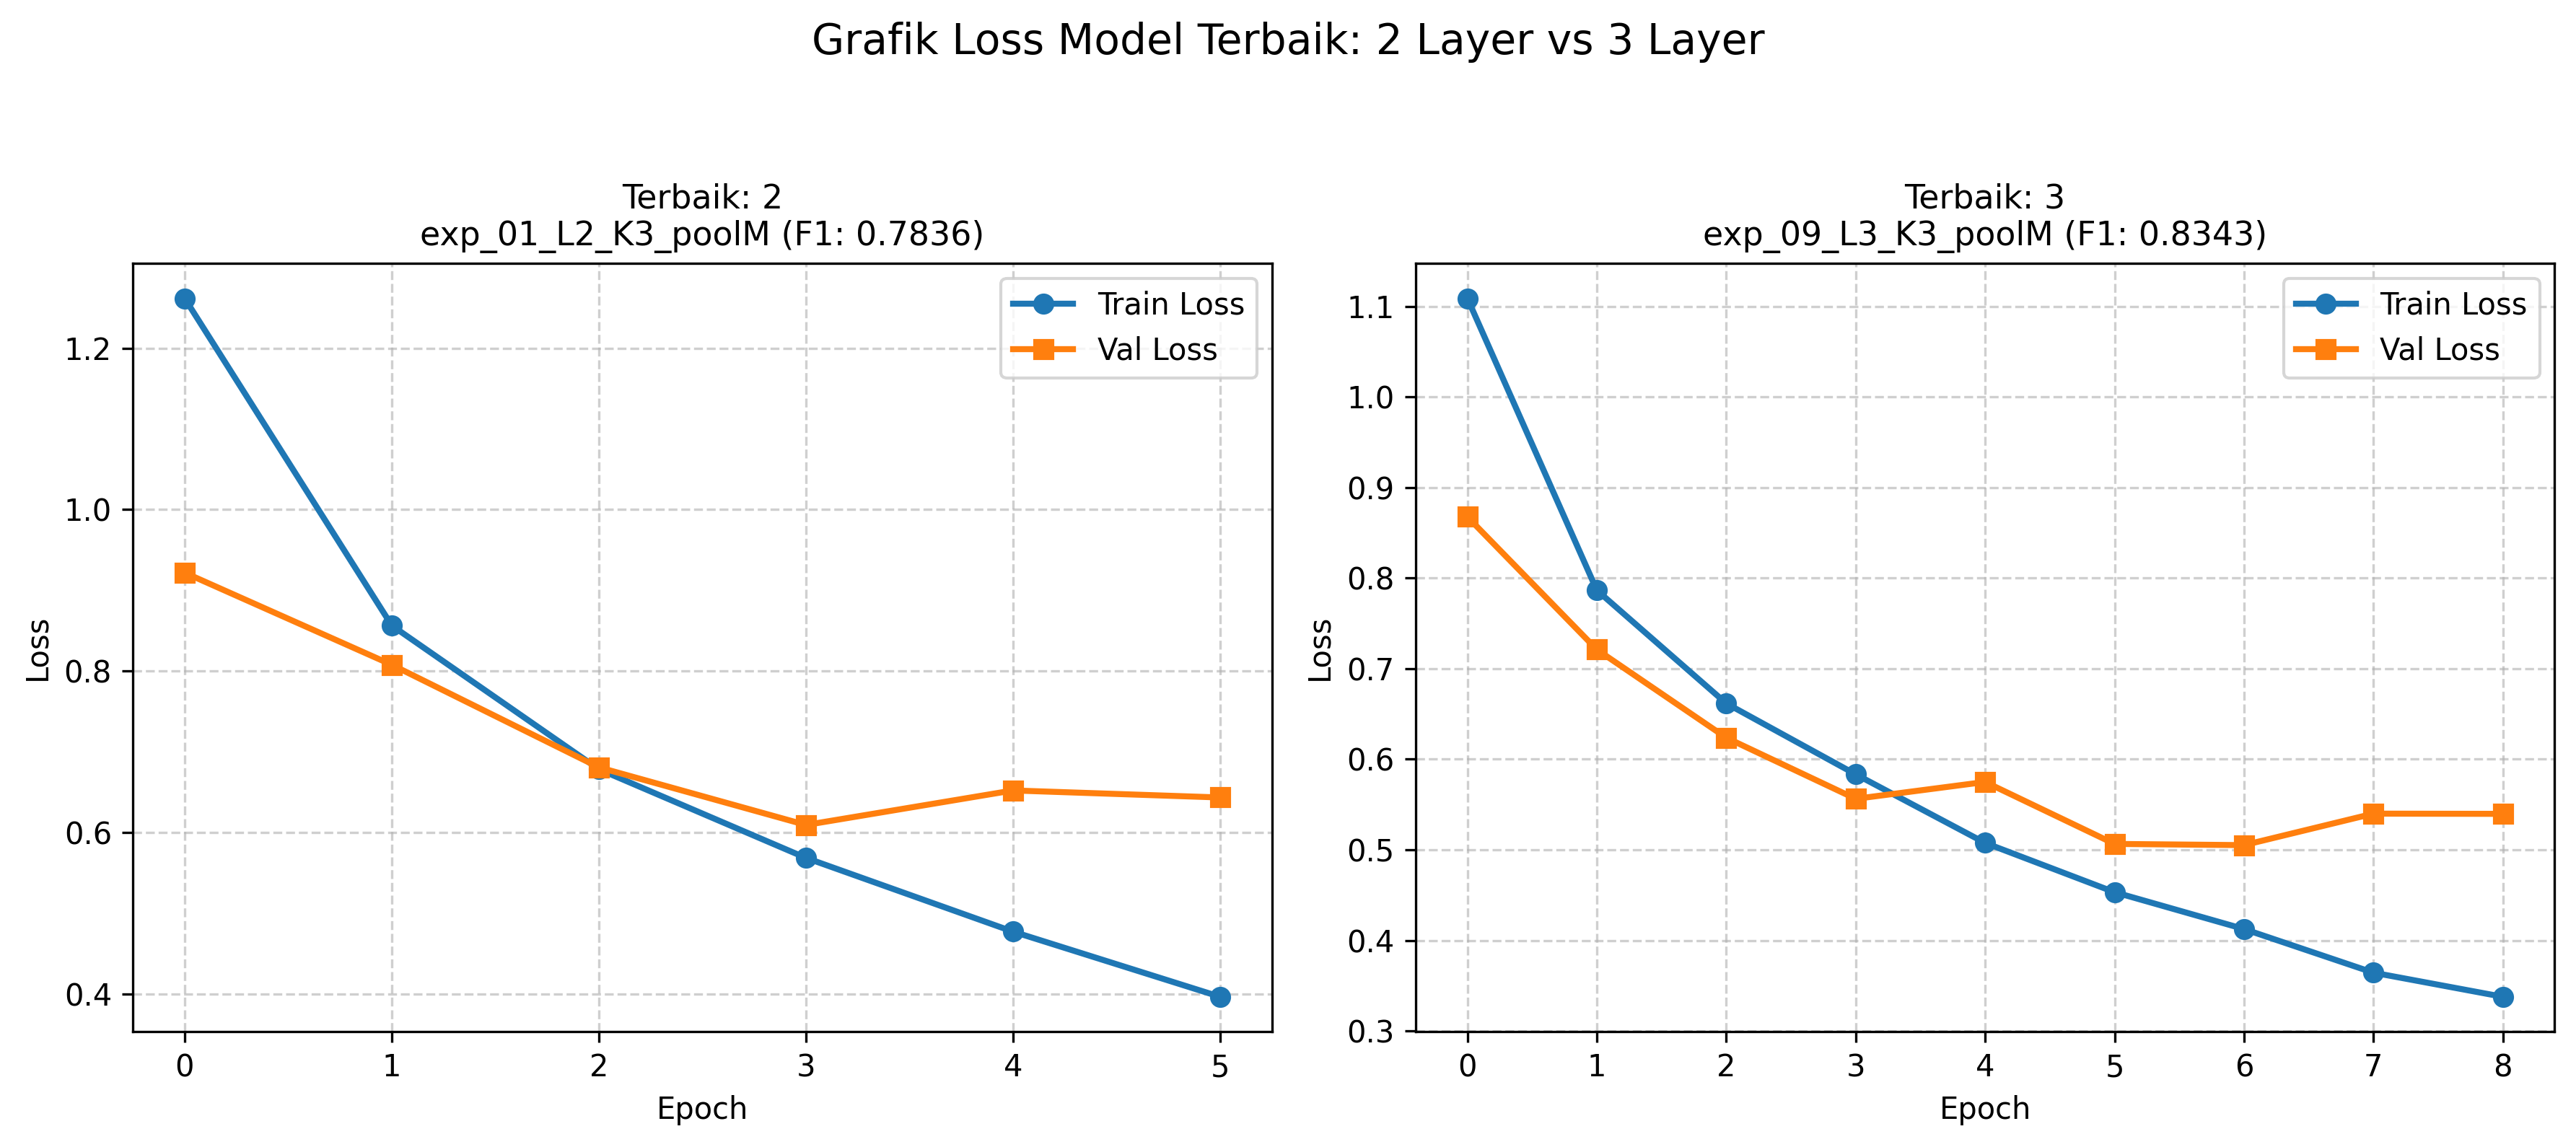
\includegraphics[width=0.9\textwidth]{assets/plot_laporan/1_Loss_Jumlah_Layer.png}
    \caption{Grafik Loss Model Terbaik: 2 Layer vs 3 Layer}
\end{figure}

\subsubsection{Pengaruh Kapasitas Model (Banyak Filter)}
Arsitektur dengan kapasitas parameter filter besar (dimulai dari 64 filter) sedikit mengungguli arsitektur filter kecil (dimulai dari 32 filter) dengan perolehan skor F1-Macro 0.7843 berbanding 0.7822. Perbedaan kinerja klasifikasi tersebut tidak terlalu eskalatif jika meninjau waktu latih yang harus dibayar. Model berkapasitas besar memakan waktu komputasi nyaris dua kali lipat lebih lama (191.80 detik) dibandingkan model yang lebih ringan (99.83 detik).

\begin{figure}[H]
    \centering
    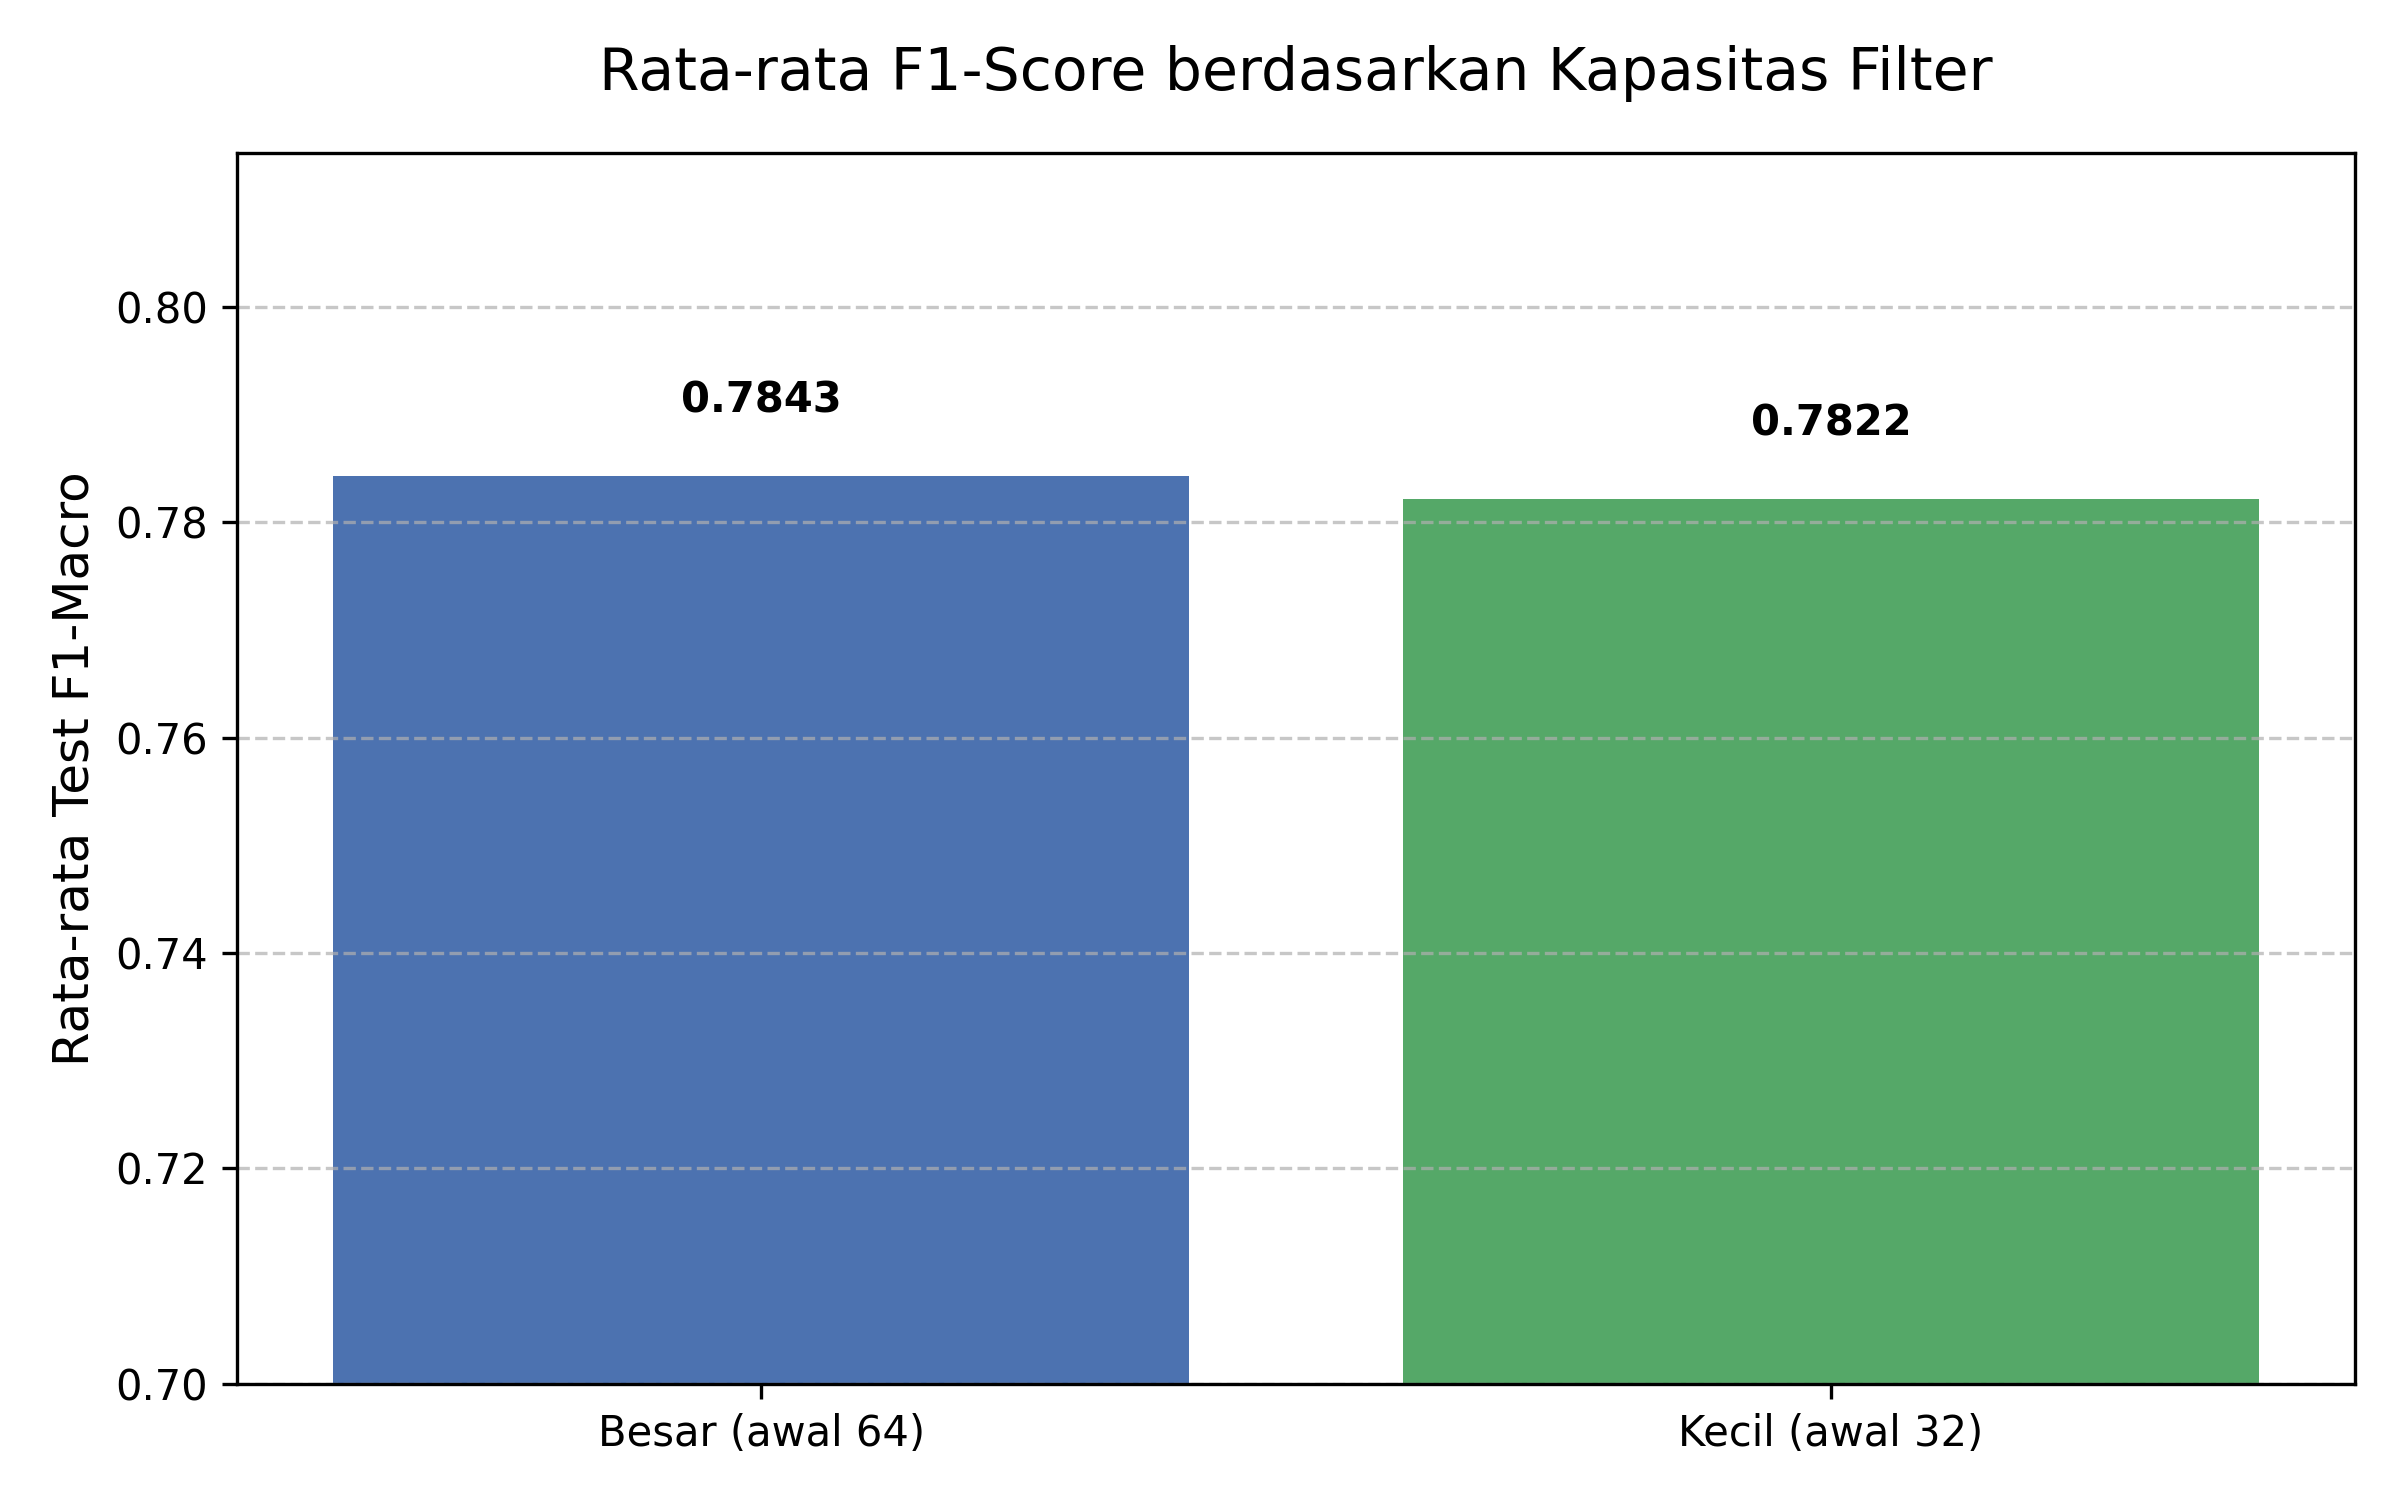
\includegraphics[width=0.7\textwidth]{assets/plot_laporan/2_F1_Kapasitas_Filter.png}
    \caption{Rata-rata F1-Score berdasarkan Kapasitas Filter}
\end{figure}
\begin{figure}[H]
    \centering
    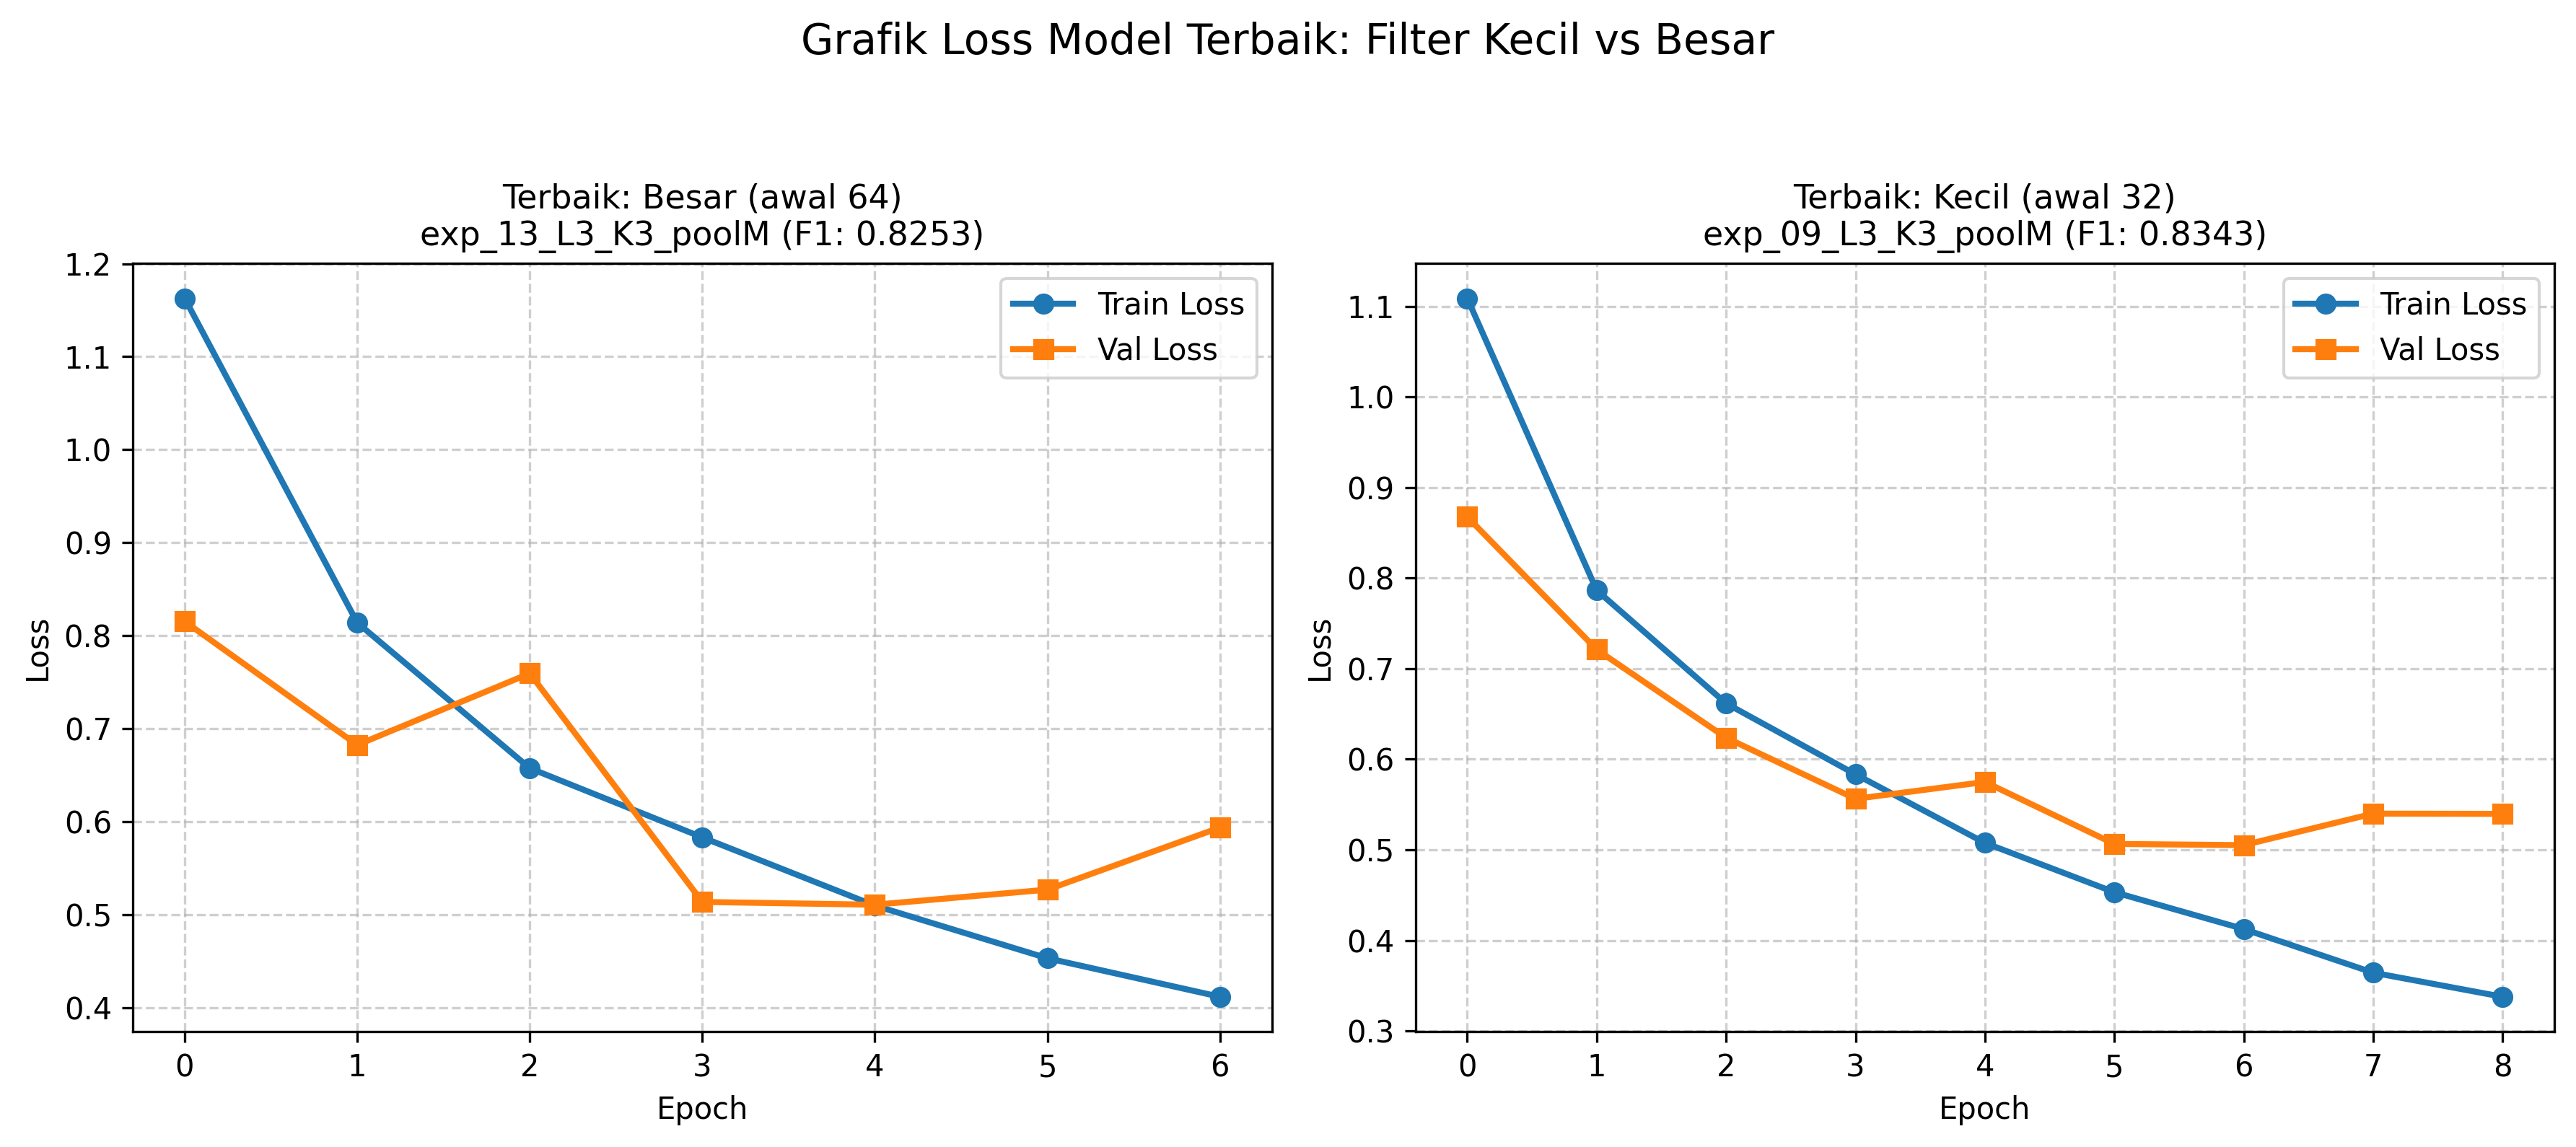
\includegraphics[width=0.9\textwidth]{assets/plot_laporan/2_Loss_Kapasitas_Filter.png}
    \caption{Grafik Loss Model Terbaik: Filter Kecil vs Besar}
\end{figure}

\subsubsection{Pengaruh Ukuran Kernel}
Eksperimen membuktikan bahwa penggunaan resolusi kernel konvolusi $3 \times 3$ memberikan performa yang jauh lebih baik (F1-Macro 0.7912) daripada agregasi informasi lebih besar yang dilakukan oleh ukuran $5 \times 5$ (F1-Macro 0.7753). Kernel $3 \times 3$ lebih unggul menangkap detail spasial. Model dengan kernel $3 \times 3$ juga lebih hemat waktu komputasi latih (117.63 detik berbanding 174.00 detik).

\begin{figure}[H]
    \centering
    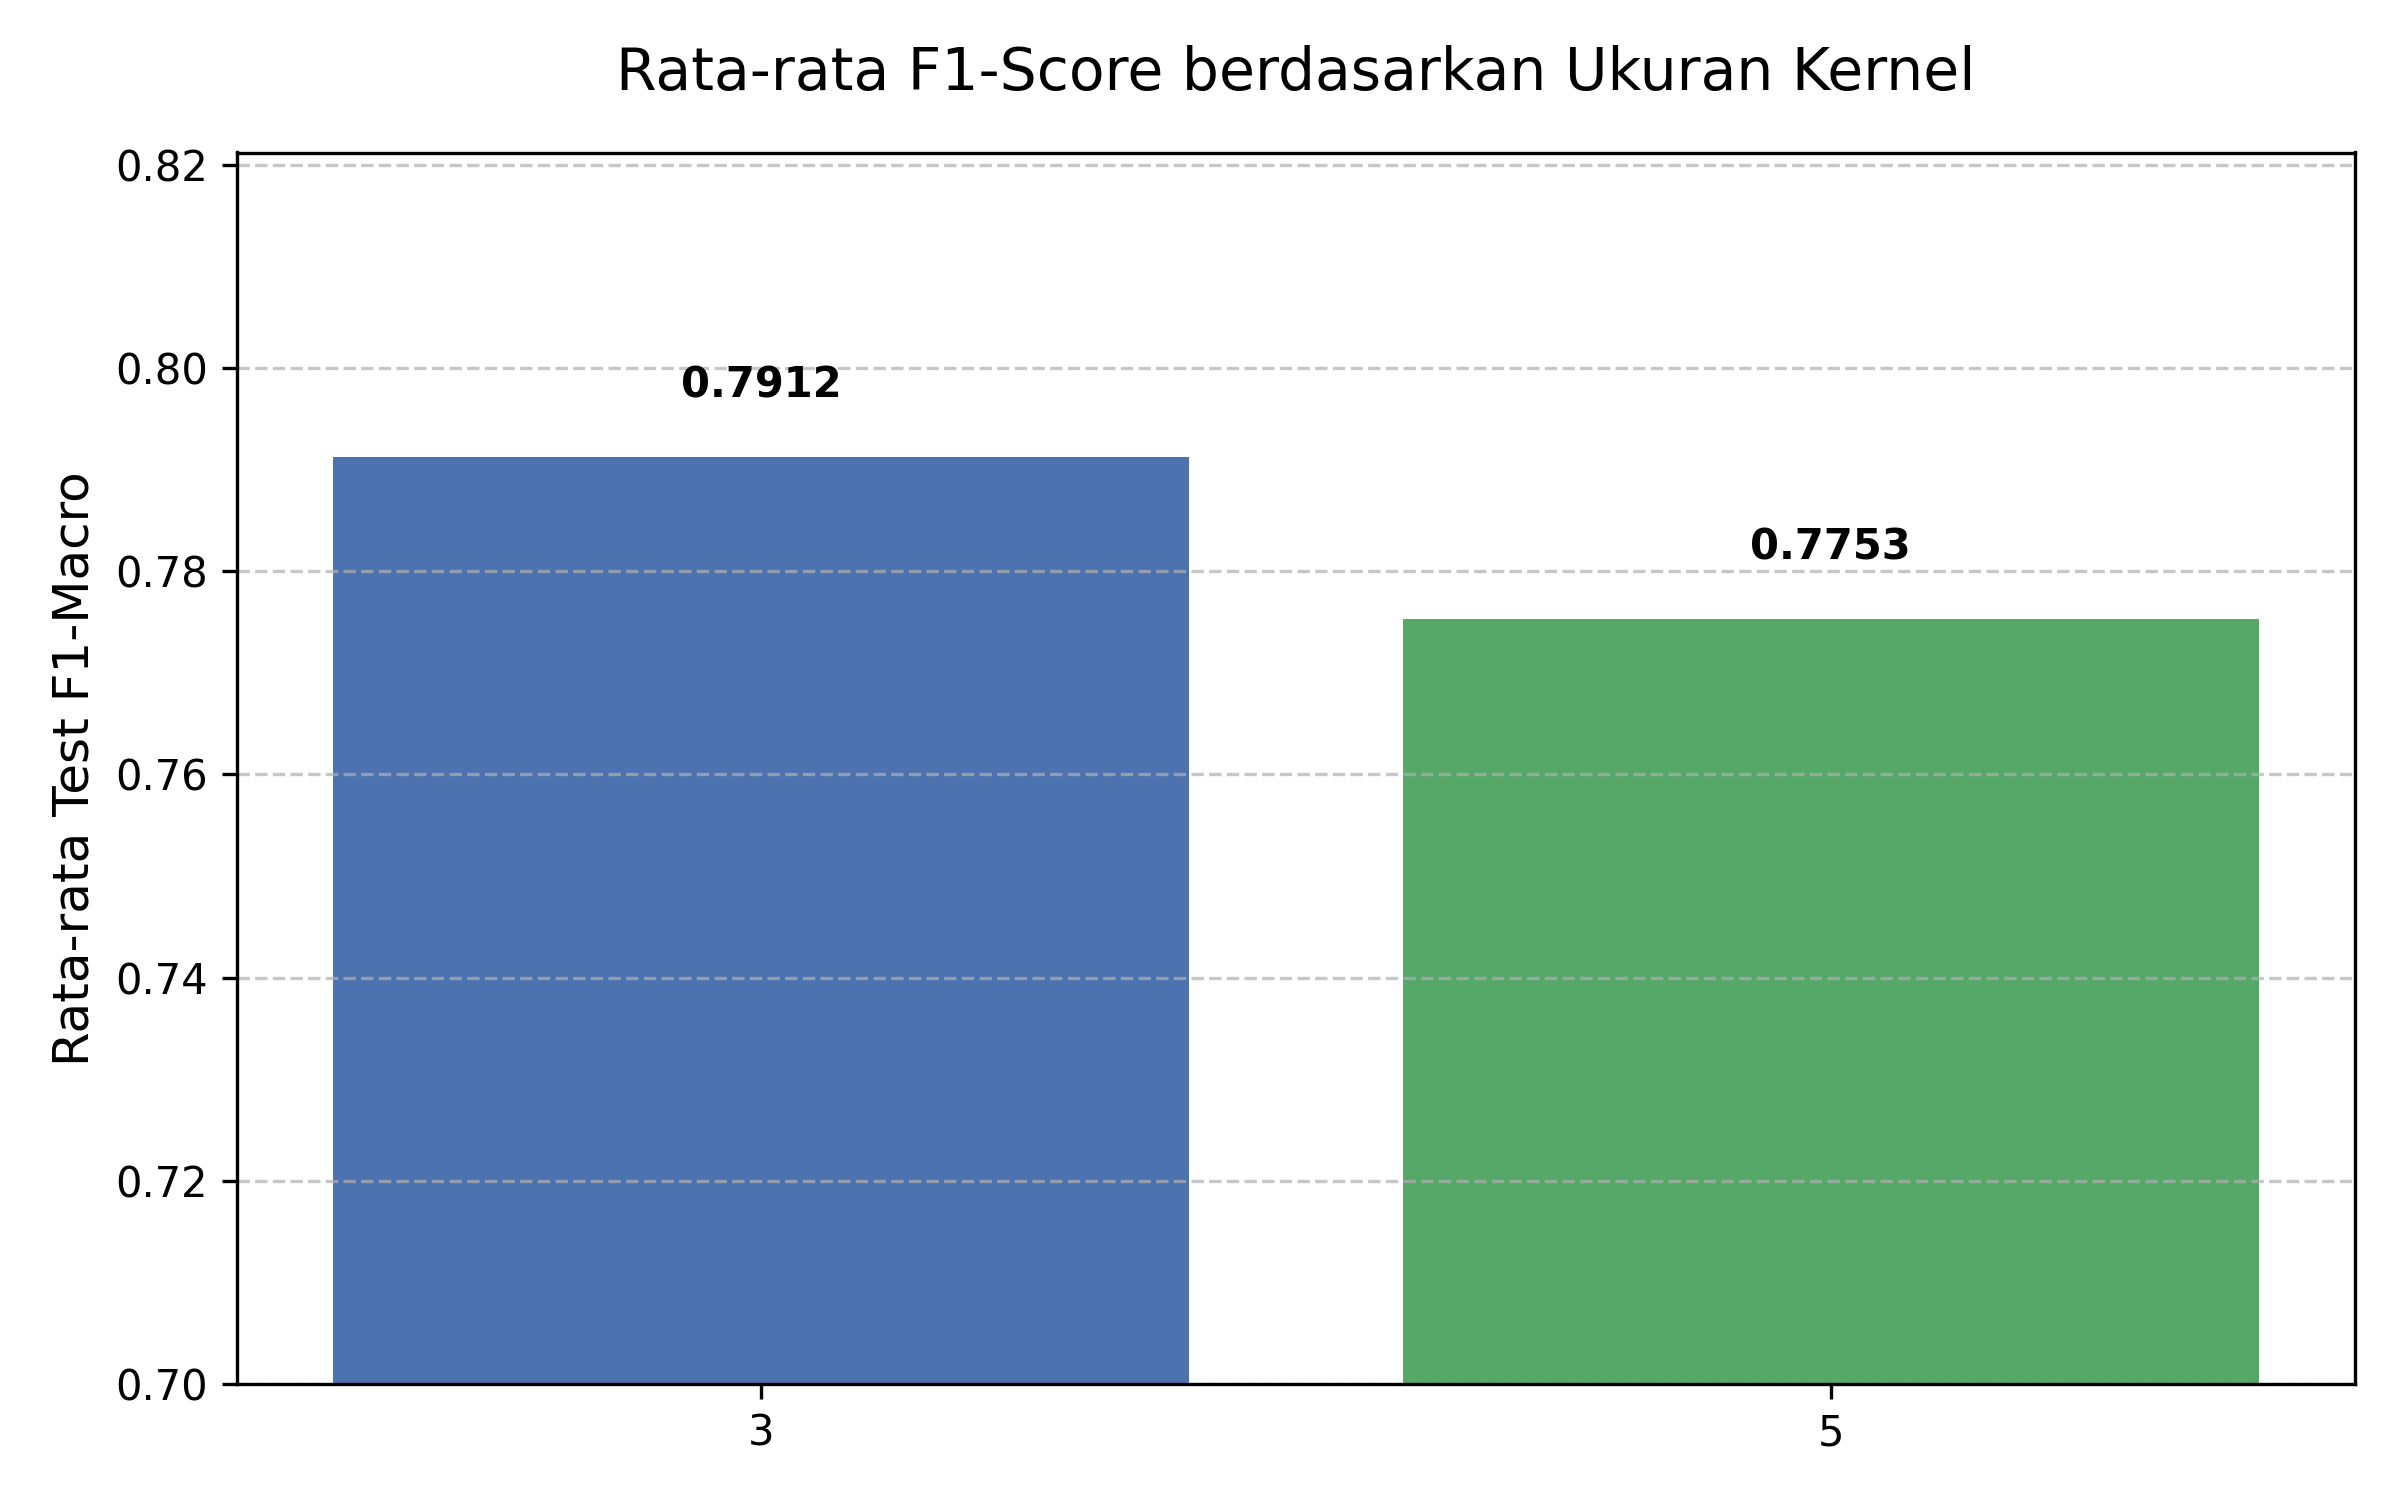
\includegraphics[width=0.7\textwidth]{assets/plot_laporan/3_F1_Ukuran_Kernel.png}
    \caption{Rata-rata F1-Score berdasarkan Ukuran Kernel}
\end{figure}
\begin{figure}[H]
    \centering
    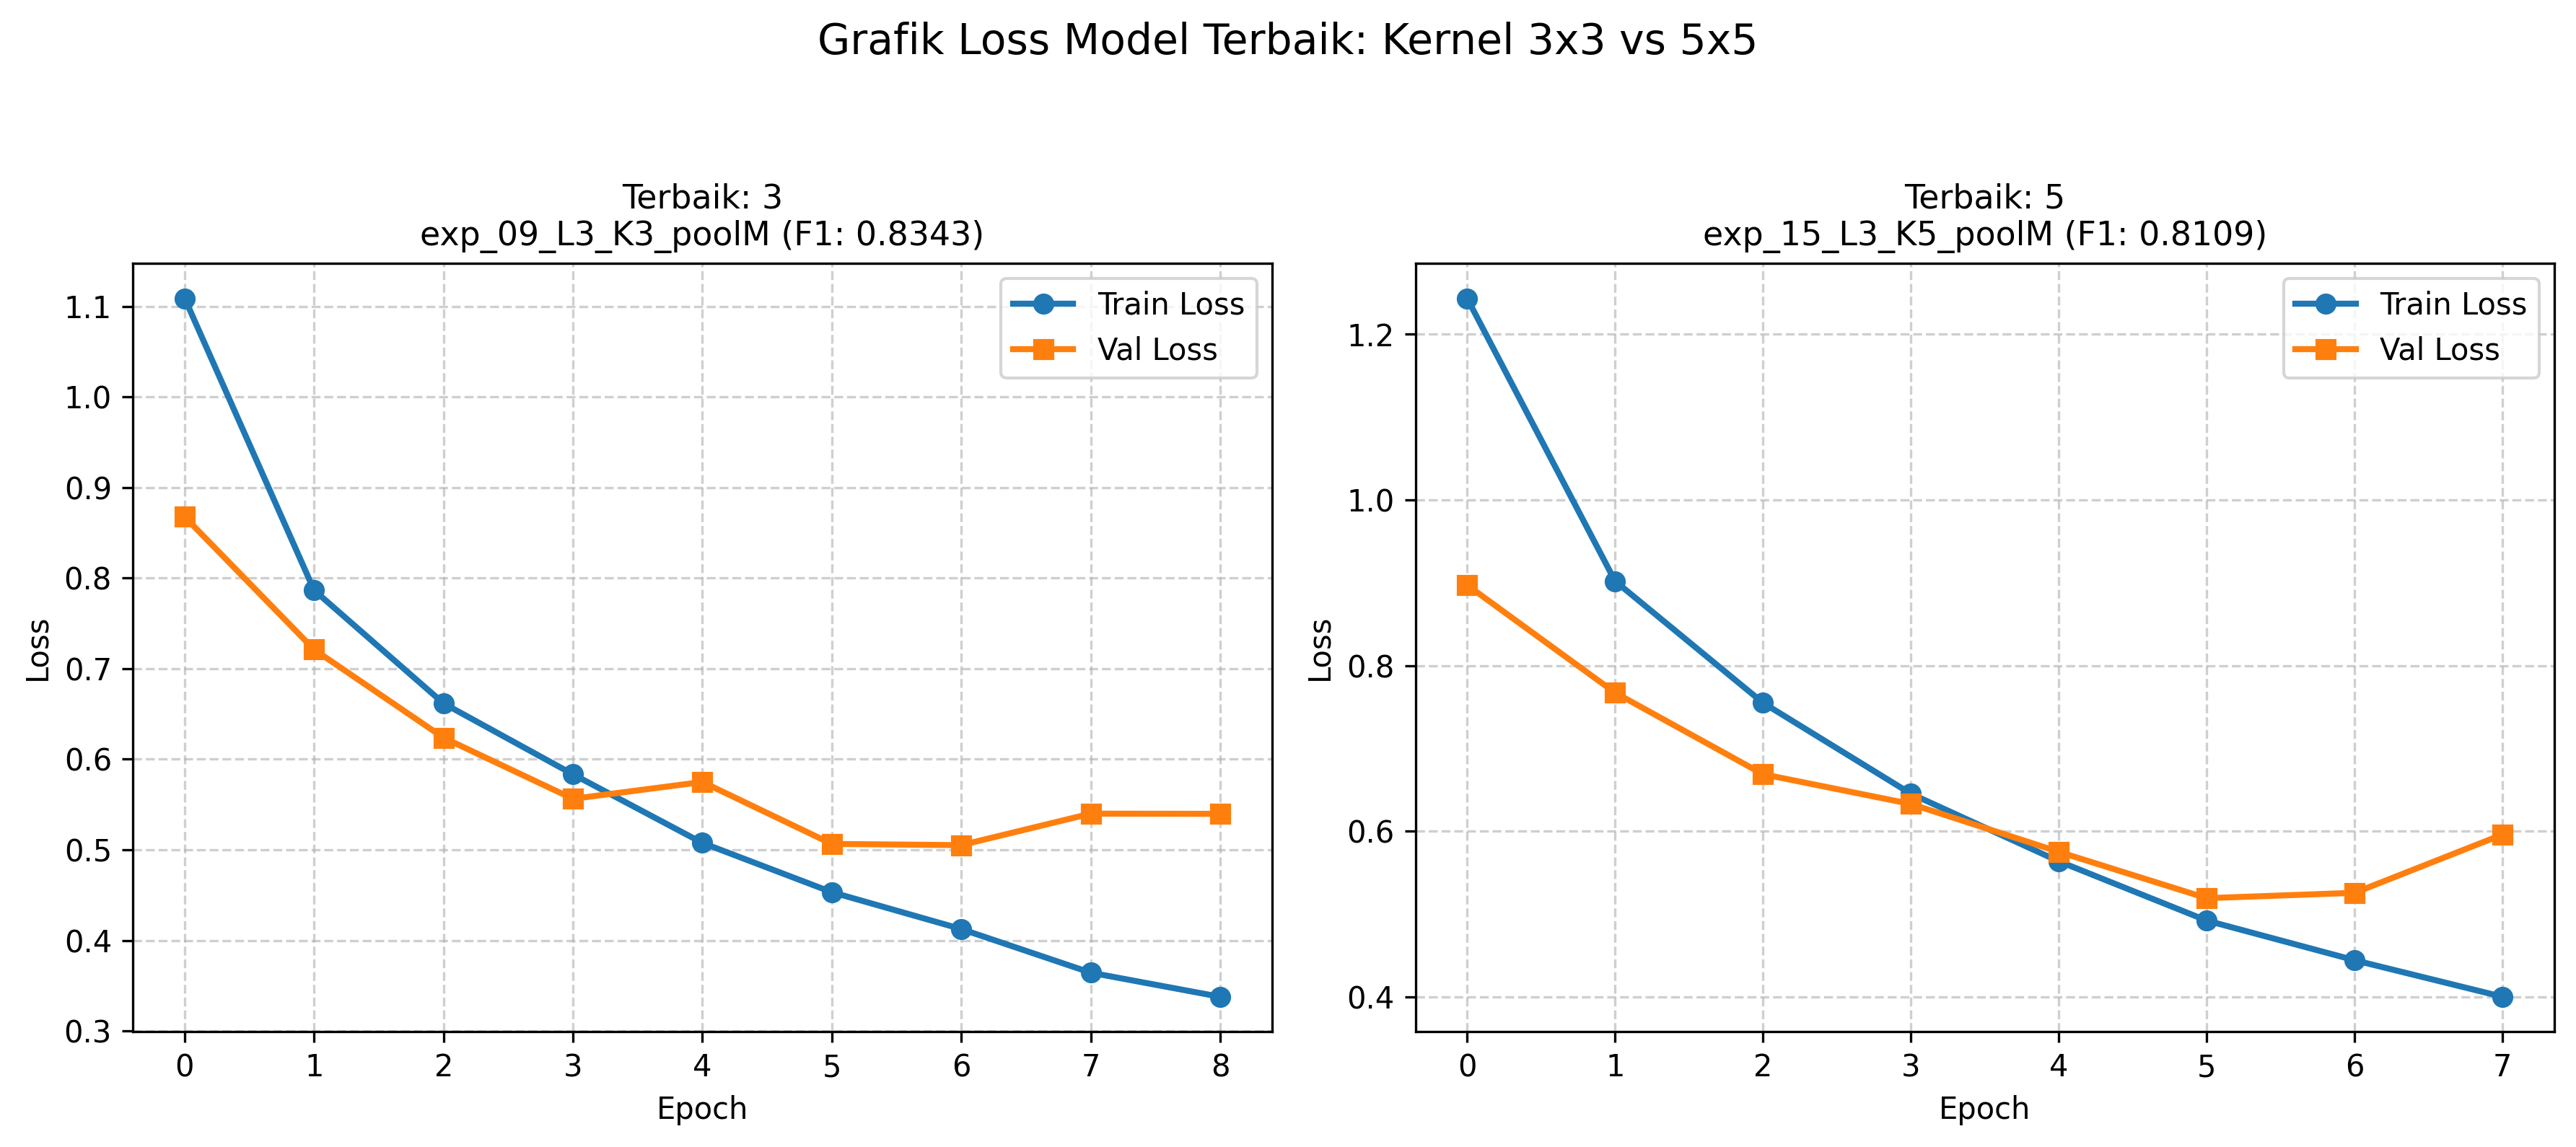
\includegraphics[width=0.9\textwidth]{assets/plot_laporan/3_Loss_Ukuran_Kernel.png}
    \caption{Grafik Loss Model Terbaik: Ukuran Kernel $3 \times 3$ vs $5 \times 5$}
\end{figure}

\subsubsection{Pengaruh Jenis Pooling Layer}
Model klasifikasi yang menerapkan \textit{Max Pooling} secara rata-rata lebih superior (F1-Macro 0.7913) bila disandingkan dengan penerapan \textit{Average Pooling} (0.7752). Hal ini dikarenakan operasi max meretensi nilai intensitas terkuat dari kumpulan fitur ketimbang meratakannya secara menyeluruh. \textit{Max pooling} berjalan dengan rerata waktu latih 157.54 detik.

\begin{figure}[H]
    \centering
    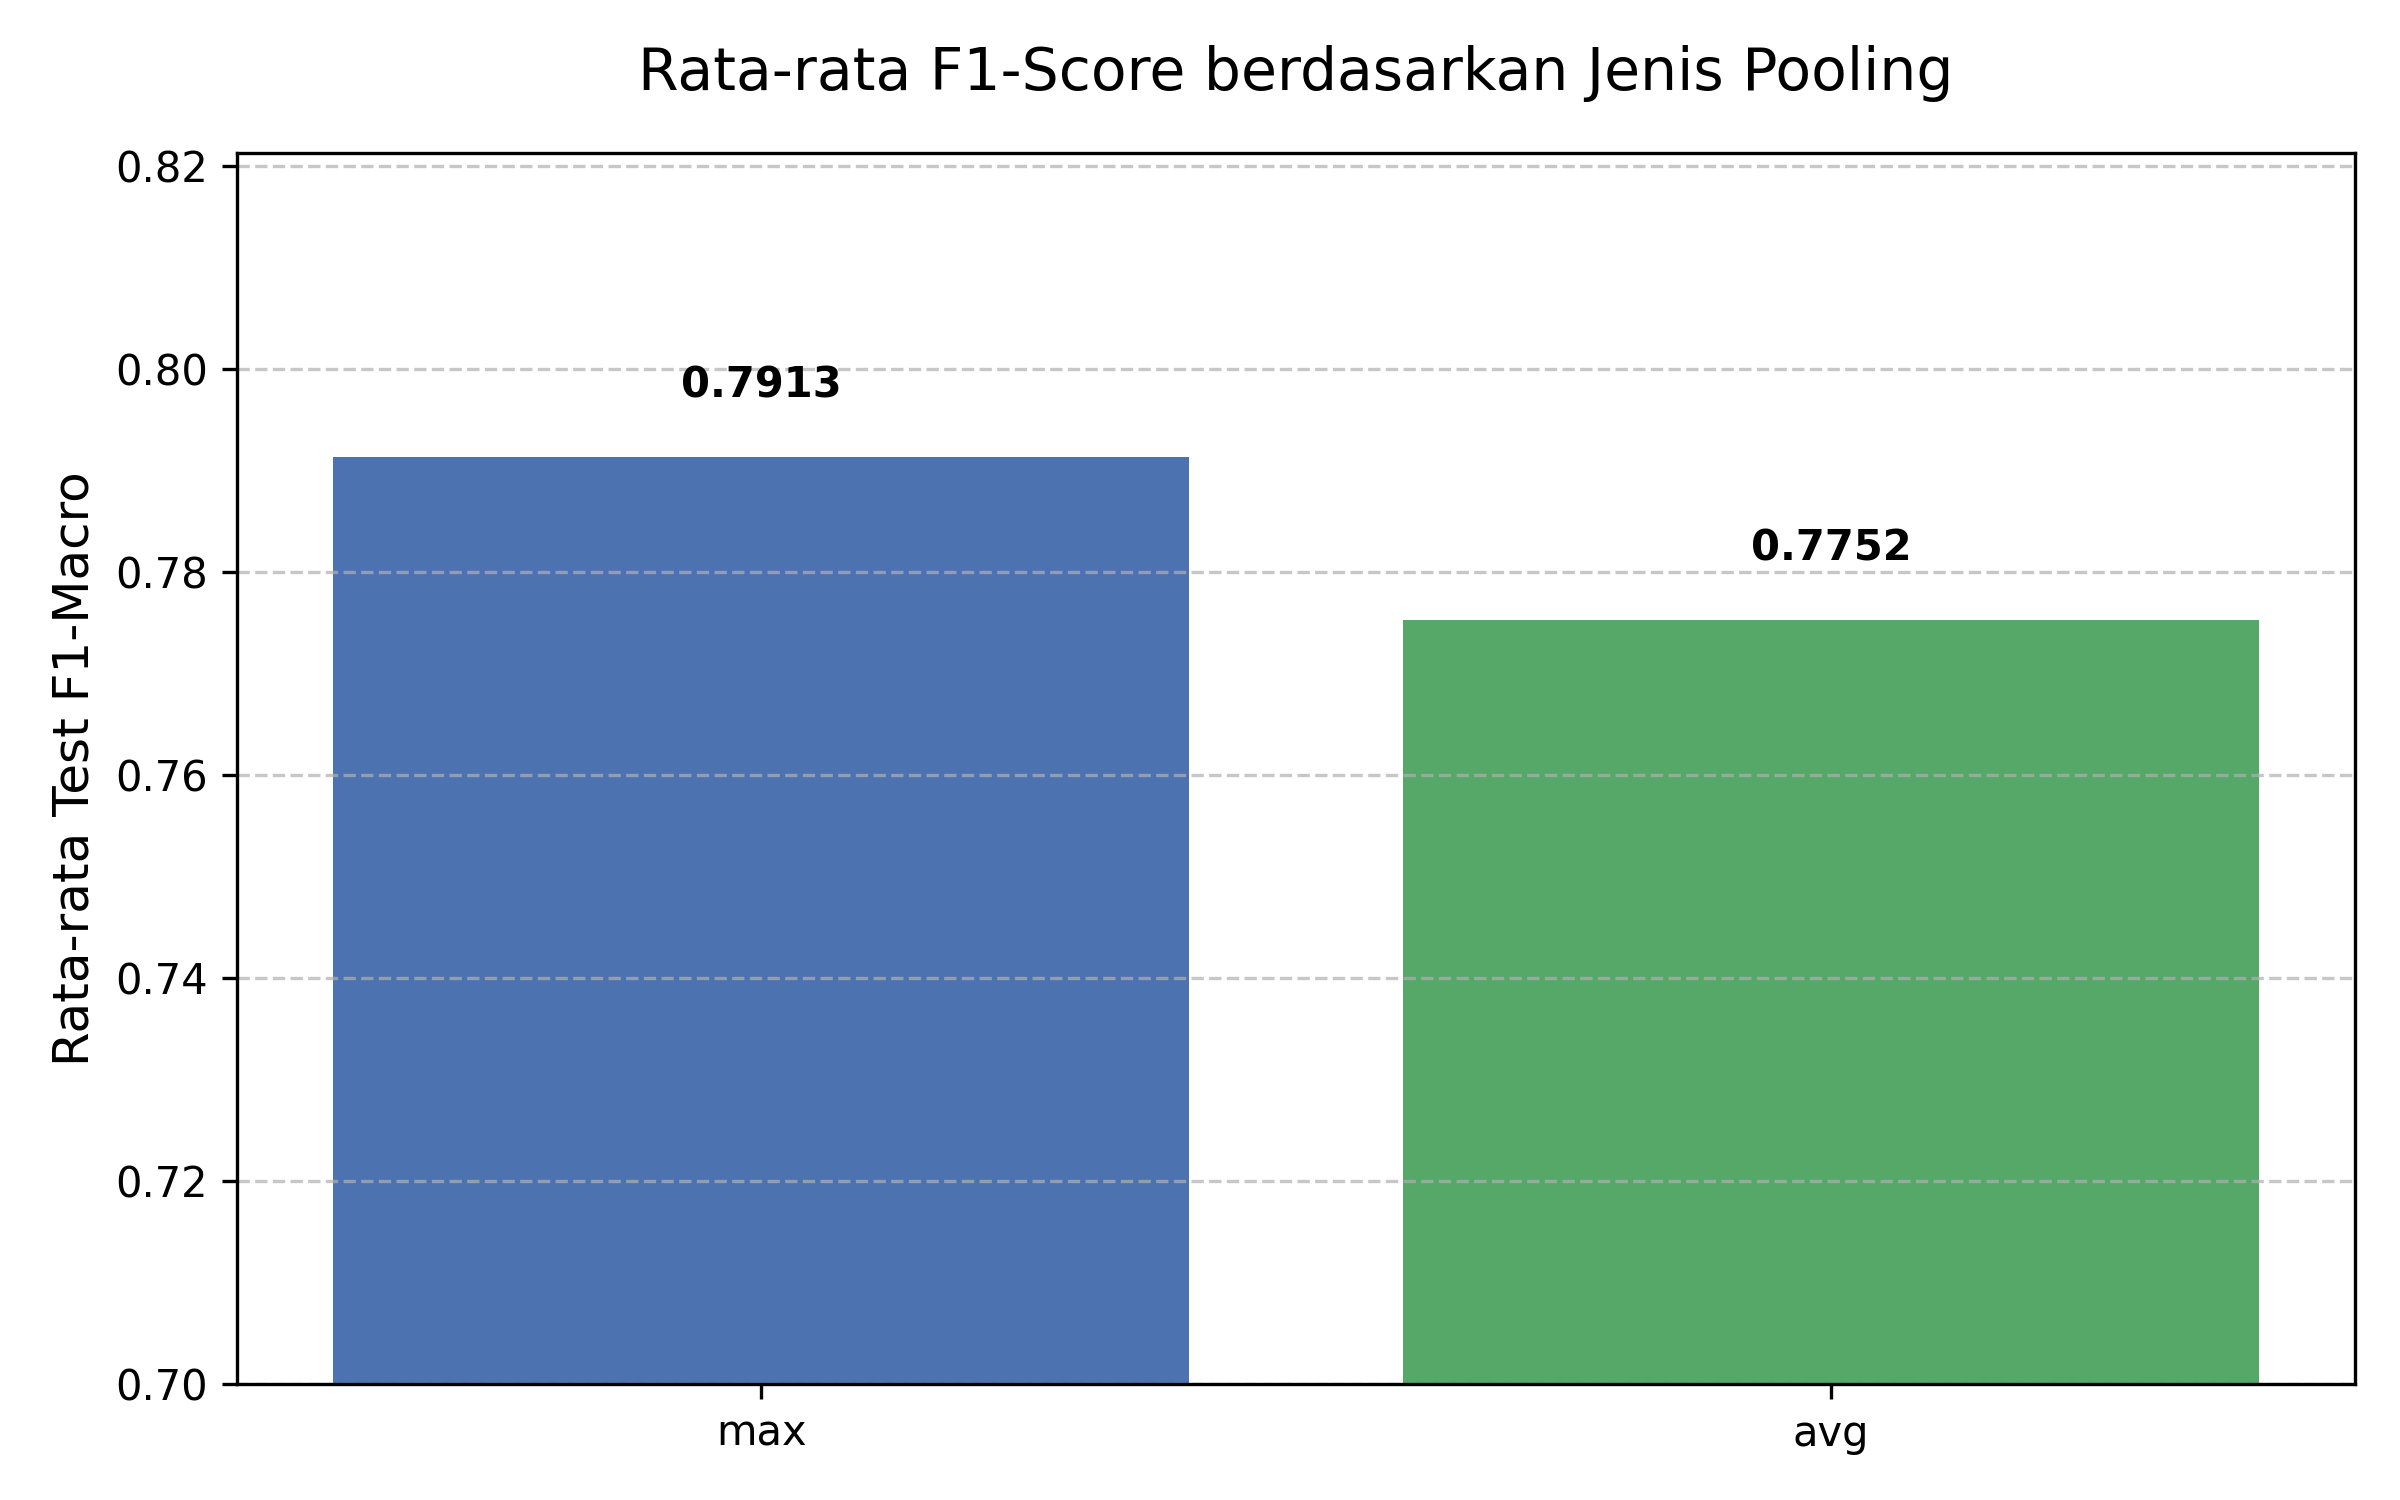
\includegraphics[width=0.7\textwidth]{assets/plot_laporan/4_F1_Jenis_Pooling.png}
    \caption{Rata-rata F1-Score berdasarkan Jenis Pooling Layer}
\end{figure}
\begin{figure}[H]
    \centering
    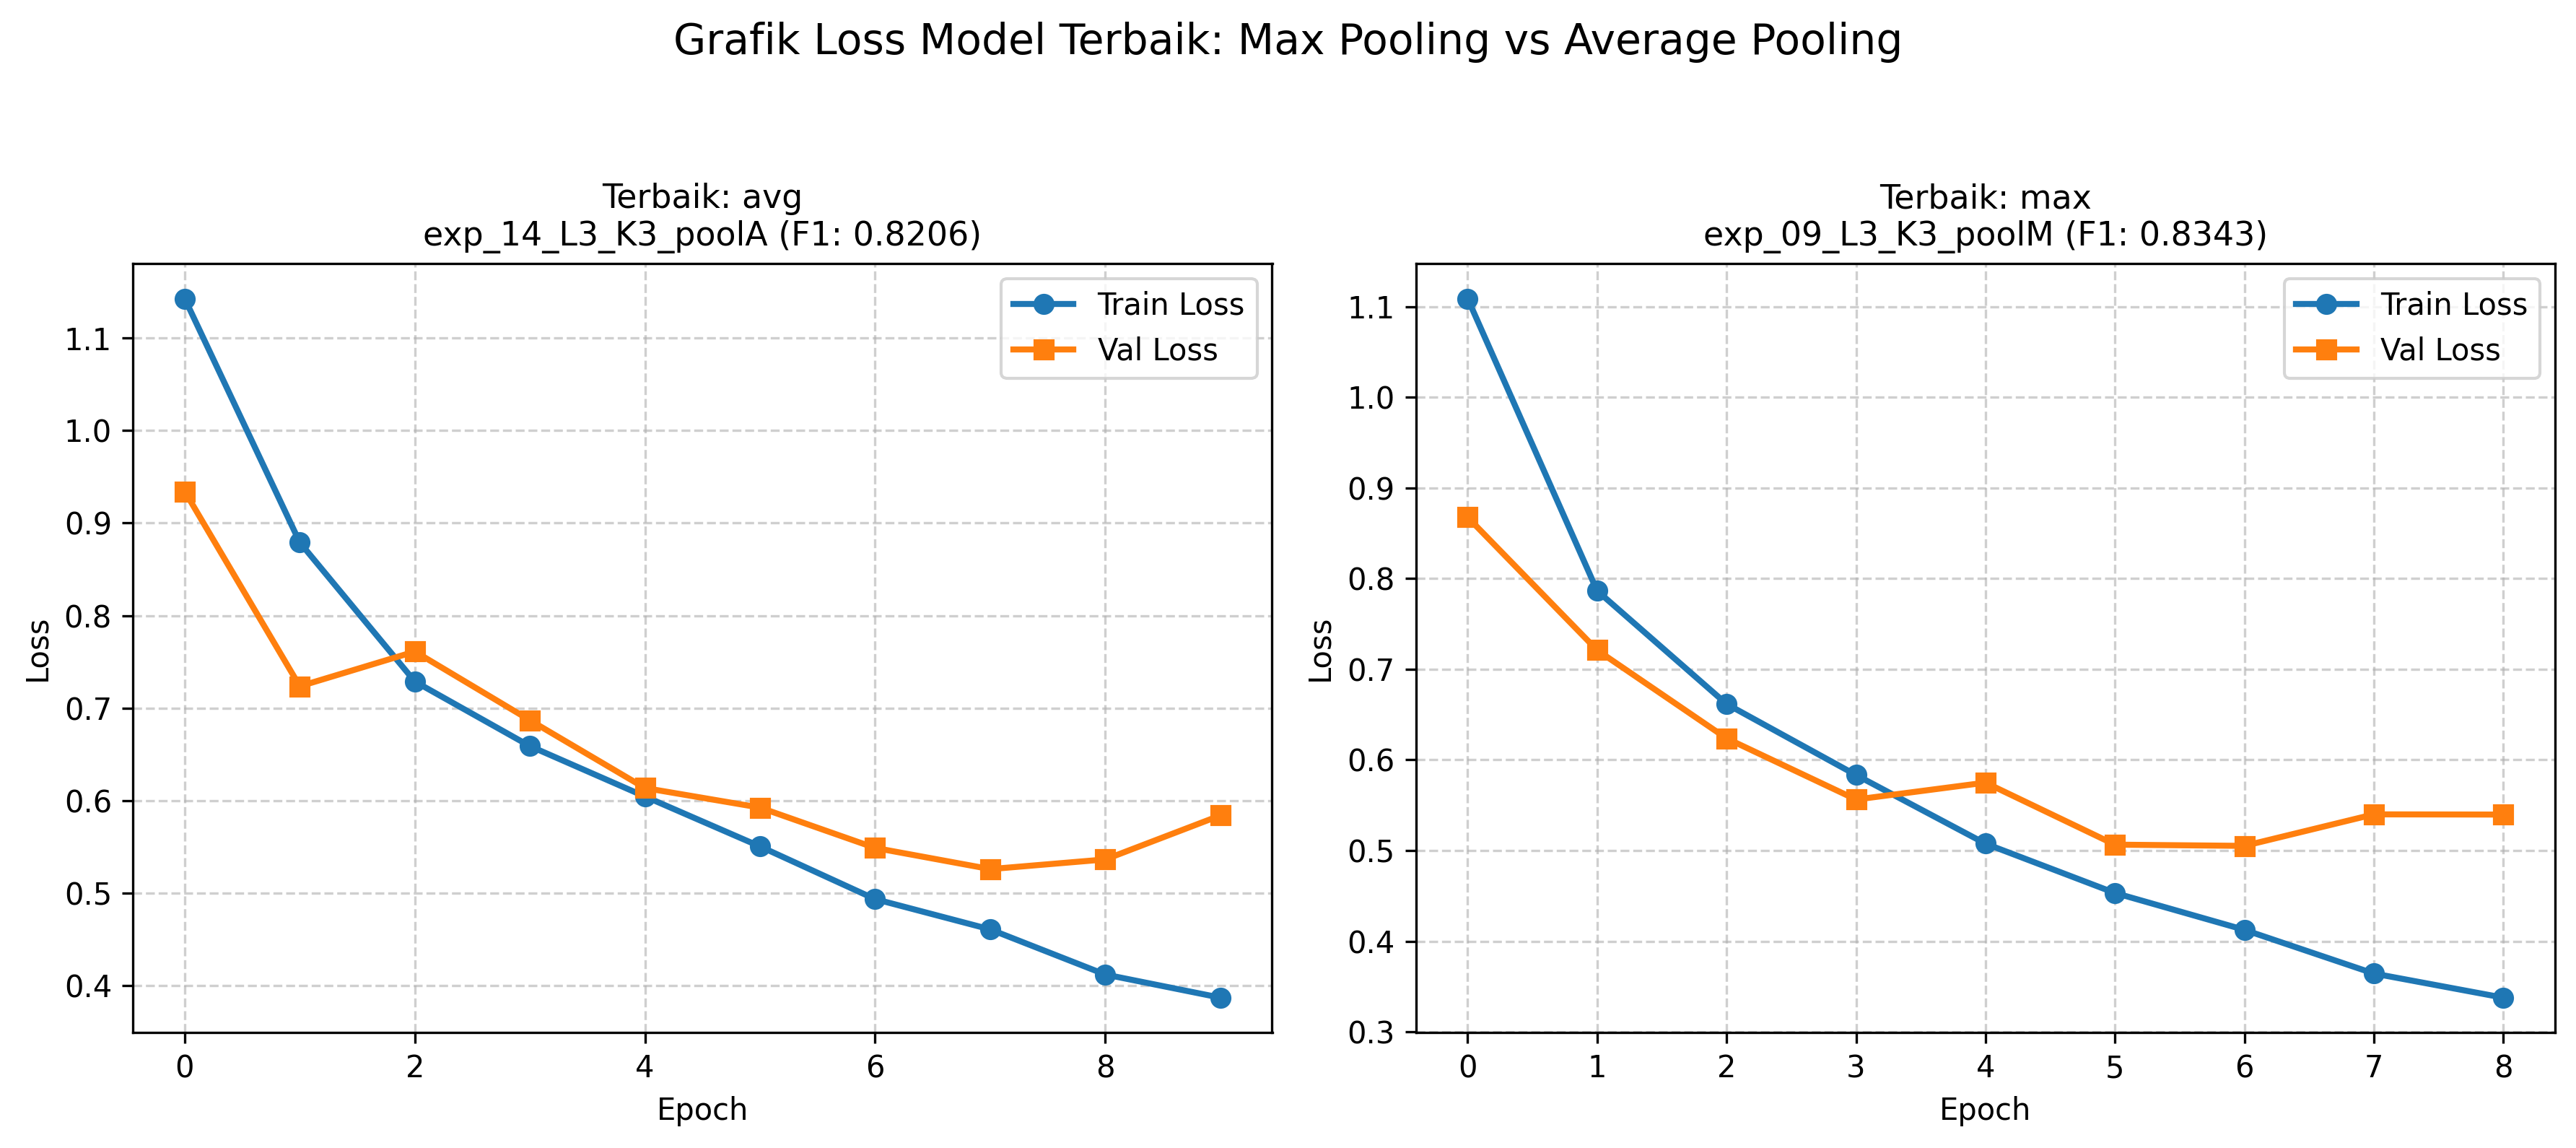
\includegraphics[width=0.9\textwidth]{assets/plot_laporan/4_Loss_Jenis_Pooling.png}
    \caption{Grafik Loss Model Terbaik: Max Pooling vs Average Pooling}
\end{figure}

\subsubsection{Perbandingan Keras vs \textit{From Scratch}}


\subsubsection{Perbandingan Arsitektur \textit{Shared} vs \textit{Non-shared}}


\subsection{Simple RNN dan LSTM}
\subsubsection{Perbandingan RNN dan LSTM}

\subsubsection{Perbandingan dengan Keras}

\subsubsection{Pengaruh Panjang Maksimum Caption terhadap BLEU-4}
